%!TEX root = /Users/louis/Documents/PhD/Deliverables/Thesis/thesis.tex
\section[Evaluating Co-Evolution Tools with an Example from UML][Evaluating Co-Evolution Tools (UML)]{Evaluating Co-Evolution Tools with an Example from UML}
\label{sec:ttc}
In contrast to the previous section, which compared Flock to three co-evolution tools, the evaluation performed in this section compares Flock with model-to-model transformation tools. As discussed in Chapter~\ref{Analysis}, model migration can be regarded as a specialisation of model-to-model transformation. Chapter~\ref{Implementation} introduces Flock, a language tailored for model migration. This section compares Flock with other model-to-model transformation languages, and explores the benefits and drawbacks of treating model migration and model-to-model transformation as separate model management operations, as proposed in this thesis and by \cite{sprinkle03thesis}.

The author participated in the 2010 edition of the Transformation Tools Contest (TTC), a workshop series that seeks to compare and contrast tools for performing model and graph transformation. At TTC 2010\footnote{\url{http://www.planet-research20.org/ttc2010/index.php?Itemid=132}}, two rounds of submissions were invited: cases (transformation problems, three of which are selected by the workshop organisers) and solutions to the selected cases. The author submitted a case based on a model migration problem from a real-world example of metamodel evolution. Nine solutions were submitted for the case, including one by the author, which used Flock.

Compared to the evaluation described in Section~\ref{sec:collaborative_comparison}, the evaluation in this section compares Flock to a wider range of tools (model and graph transformation tools, and not just model migration tools). The remainder of this section describes the model migration case (Section~\ref{subsec:ttc_case}), the Flock solution (Section~\ref{subsec:ttc_solution}), and reports the results of the workshop in which the solutions were compared and scored by the organisers and participants.


\subsection{Model Migration Case}
\label{subsec:ttc_case}
To compare Flock with other transformation tools for specifying model migration, the author submitted a case to TTC based on the evolution of the UML. The way in which activity diagrams are modelled in the UML changed significantly between versions 1.4 and 2.1 of the specification. In the former, activities were defined as a special case of state machines, while in the latter they are defined with a more general semantic base\footnote{A variant of generalised coloured Petri nets.} \cite{selic05uml2}.

The remainder of this section briefly introduces UML activity diagrams, describes their evolution, and discusses the way in which solutions were assessed. Section~\ref{subsec:uml_activity_diagrams} describes the metamodel evolution in more detail. The work presented in this section is based on the case submitted to TTC 2010 \cite{rose10ttc_case}. 

\subsubsection{Activity Diagrams in UML}
Activity diagrams are used for modelling lower-level behaviours, emphasising sequencing and co-ordination conditions. They are used to model business processes and logic \cite{uml22}. Figure~\ref{fig:activity} shows an activity diagram for filling orders. The diagram is partitioned into three \emph{swimlanes}, representing different organisational units. \emph{Activities} are represented with rounded rectangles and \emph{transitions} with directed arrows. \emph{Fork} and \emph{join} nodes are specified using a solid black rectangle. \emph{Decision} nodes are represented with a diamond. Guards on transitions are specified using square brackets. For example, in Figure~\ref{fig:activity} the transition to the restock activity is guarded by the condition \texttt{[not in stock]}. Text on transitions that is not enclosed in square brackets represents a trigger event. In Figure~\ref{fig:activity}, the transition from the restock activity occurs on receipt of the asynchronous signal called \texttt{receive stock}. Finally, the transitions between activities might involve interaction with objects. In Figure~\ref{fig:activity}, the Fill Order activity leads to an interaction with an object called \texttt{Filled Object}. 

\begin{figure}[htbp]
  \centering
  \includegraphics*[viewport=75 230 585 800,width=13cm]{6.Evaluation/images/activity.pdf}
  \caption[Activity model in UML 1.4.]{Activity model in UML 1.4, taken from \cite{rose10ttc_case} and based on \cite[pg3-165]{uml14}.}
  \label{fig:activity}
\end{figure}

Between versions 1.4 and 2.2 of the UML specification, the metamodel for activity diagrams has changed significantly. The sequel summarises most of the changes, and details can be found in \cite{uml14} and \cite{uml22}.

\subsubsection{Evolution of Activity Diagrams}
Figures~\ref{fig:uml14} and \ref{fig:uml22} are simplifications of the activity diagram metamodels from versions 1.4 and 2.2 of the UML specification, respectively. In the interest of clarity, some features and abstract classes have been removed from Figures~\ref{fig:uml14} and \ref{fig:uml22}.

Some differences between Figures~\ref{fig:uml14} and \ref{fig:uml22} are: activities have been changed such that they comprise nodes and edges, actions replace states in UML 2.2, and the subtypes of control node replace pseudostates.

\begin{figure}[htbp]
  \centering
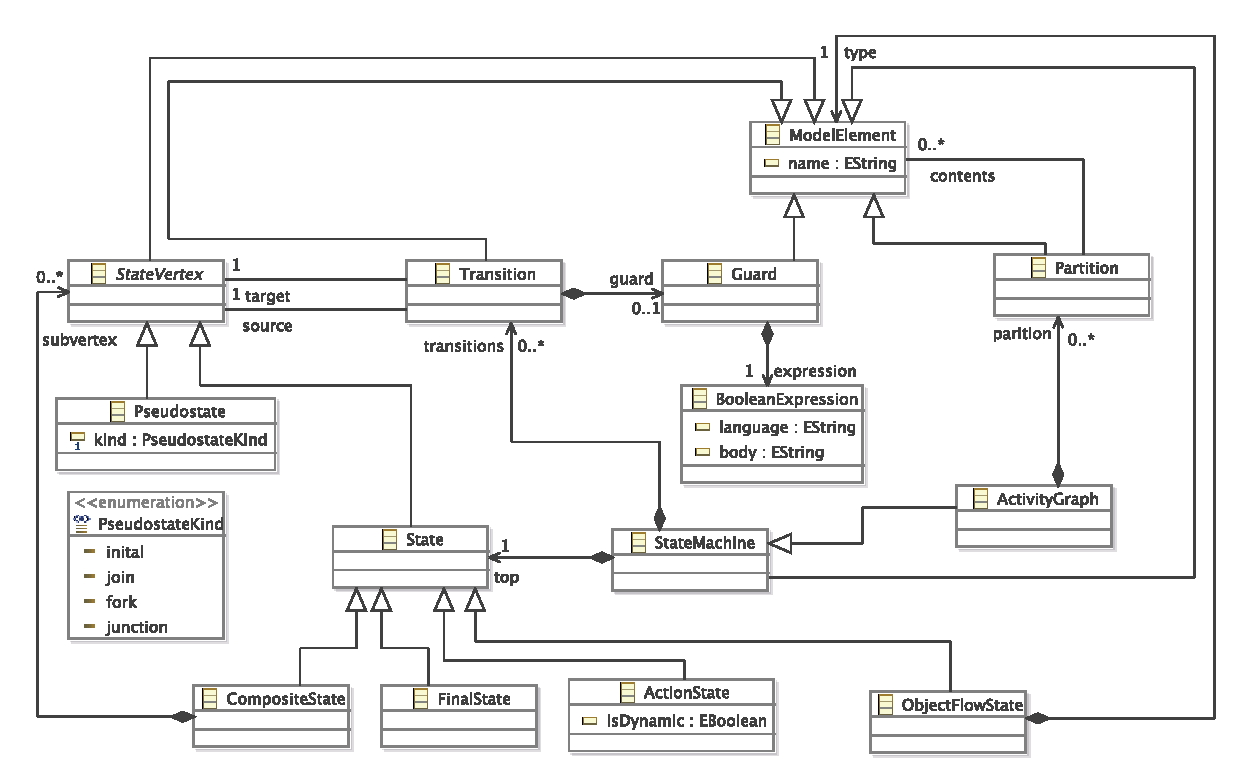
\includegraphics[width=12cm]{A.3.MigrationStrategies/images/uml/activity_diagrams_before.pdf}
  \caption[UML 1.4 Activity Graphs]{UML 1.4 Activity Graphs (based on \cite{uml14}).}
  \label{fig:uml14}
\end{figure} 

\begin{figure}[htbp]
  \centering
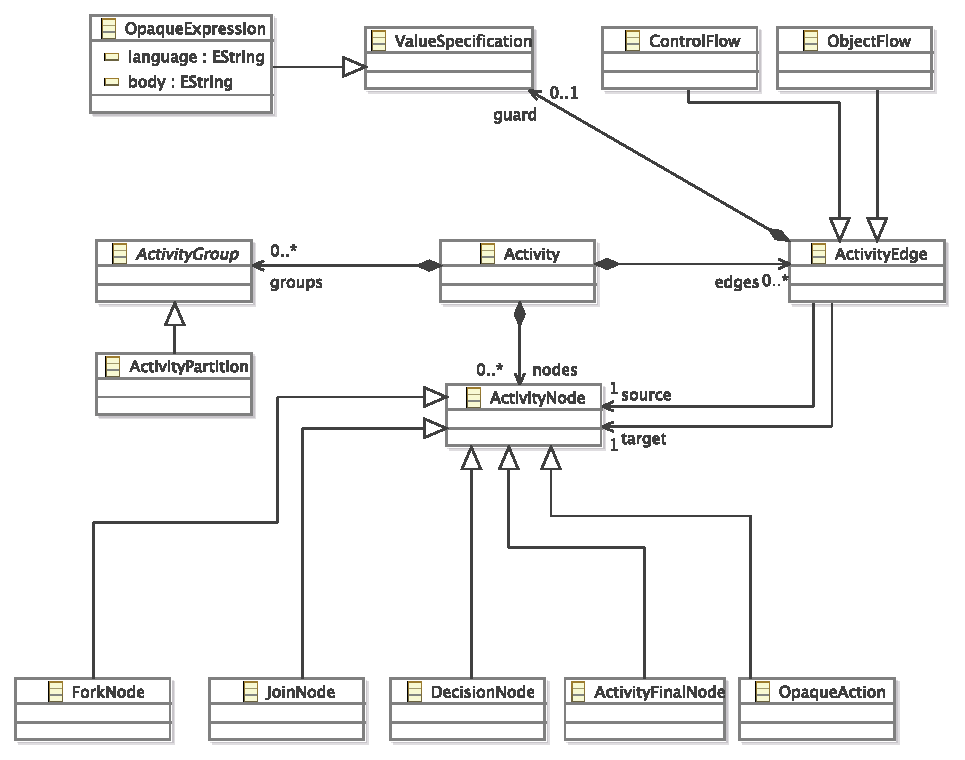
\includegraphics[width=12cm]{A.3.MigrationStrategies/images/uml/activity_diagrams_after.pdf}
  \caption[UML 2.2 Activity Diagrams]{UML 2.2 Activity Diagrams (based on \cite{uml22}).}
  \label{fig:uml22}
\end{figure}

To facilitate the comparison of solutions, the model shown in Figure~\ref{fig:activity} was used. Solutions migrated the activity diagram shown in Figure~\ref{fig:activity} -- which conforms to UML 1.4 -- to conform to UML 2.2. The UML 1.4 model, the migrated UML 2.2 model, and the UML 1.4 and 2.2 metamodels are available from\footnote{\url{http://www.cs.york.ac.uk/~louis/ttc/}}.

Submissions were evaluated using the following four criteria, which were decided in advance by the author and the workshop organisers:

\begin{itemize}
	\item \textbf{Correctness}: Does the transformation produce a model equivalent to the migrated UML 2.2. model included in the case resources?
	\item \textbf{Conciseness}: How much code is required to specify the transformation? (In \cite{sprinkle04domain} et al. propose that the amount of effort required to codify migration should be directly proportional to the number of changes between original and evolved metamodel).
		\item \textbf{Clarity}: How easy is it to read and understand the used transformation? (For example, is a well-known or standardised language?)
		\item \textbf{Appropriateness}: How much effort is required to adapt the tool in providing a solution?
		\item \textbf{Tool maturity}: To what extent can the tool be used by people other than the developer? 
		\item \textbf{Reproducibility}: Can the solution be reproduced on another machine?\footnote{Participants were invited to install their tools and solutions on virtual machines, which would later be made accessible via the workshop proceedings.}
		\item \textbf{Extensions}: Which of the case extensions (described below) were implemented in the solution?
\end{itemize}

To further distinguish between solutions, three extensions to the core task were proposed. The first extension was added after the case was submitted, and was proposed by the workshop organisers and the solution authors. The second and third extension were included in the case by the author. 

\subsubsection{Extension 1: Alternative Object Flow State Migration Semantics}
\label{sub:object_flow_states}
Following the submission of the case to the competition, discussion on the TTC forums\footnote{\url{http://planet-research20.org/ttc2010/index.php?option=com_community&view=groups&task=viewgroup&groupid=4&Itemid=150} (registration required)} revealed an ambiguity in the UML 2.2 specification indicating that the migration semantics for the ObjectFlowState UML 1.4 concept are not clear from the UML 2.2 specification. The case was revised to incorporate both the original semantics (suggested by the author and described above) and an alternative semantics (suggested by a workshop participant via the TTC forums) for migrating ObjectFlowStates. The alternative semantics are now described.

\textbf{In the core task} described above, instances of \texttt{Ob\-je\-ctFl\-owSt\-a\-te} were migrated to instances of \texttt{Ob\-je\-ctNo\-de}. Any instances of \texttt{Tr\-an\-si\-ti\-on} that had an \texttt{Ob\-je\-ctFl\-owSt\-a\-te} as their source or target were migrated to instances of \texttt{Ob\-je\-ctFl\-ow}. Figure~\ref{fig:ofs_to_node} shows an example application of this migration semantics. Structures such as the one shown in Figure~\ref{fig:ofs_to_node_before} are migrated to an equivalent structure shown in Figure~\ref{fig:ofs_to_node_after}. The \texttt{Tr\-an\-si\-ti\-on}s, \texttt{t1} and \texttt{t2}, are migrated to instances of \texttt{Ob\-je\-ctFl\-ow}. Likewise, the instance of \texttt{Ob\-je\-ctFl\-owSt\-a\-te}, \texttt{s2}, is migrated to an instance of \texttt{Ob\-je\-ctNo\-de}.

\begin{figure}[htbp]
	\centering
	\subfigure[ObjectFlowState structure in UML 1.4]
	{
	    \label{fig:ofs_to_node_before}
	    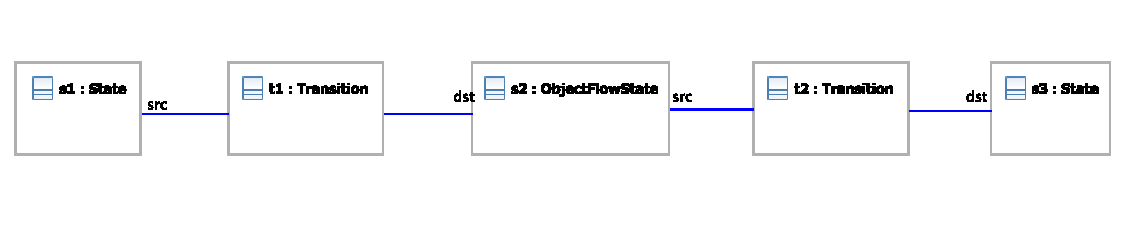
\includegraphics[height=2.5cm]{6.Evaluation/images/ttc/core_before.pdf}
	}
	\subfigure[Equivalent ObjectNode structure in UML 2.2]
	{
	    \label{fig:ofs_to_node_after}
	    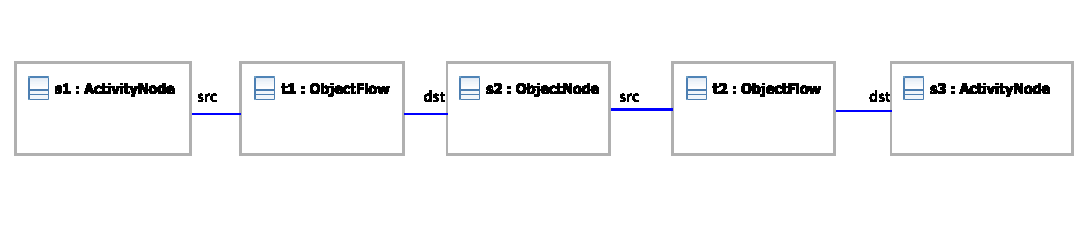
\includegraphics[height=2.5cm]{6.Evaluation/images/ttc/core_after.pdf}
	}
	\caption{Migrating Actions for the Core Task}
\label{fig:ofs_to_node}
\end{figure}


\textbf{This extension} considered an alternative migration semantics for ObjectFlowState. For this extension, instances of \texttt{Ob\-je\-ctFl\-owSt\-a\-te} (and any connected \texttt{Tr\-an\-si\-ti\-on}s) were migrated to instances of  \texttt{Ob\-je\-ctFl\-ow}, as shown in Figure~\ref{fig:ofs_to_flow} in which the UML 2.2 \texttt{Ob\-je\-ctFl\-ow}, \texttt{f1}, replaces \texttt{t1}, \texttt{t2} and \texttt{s2}.

\begin{figure}[htbp]
	\centering
	\subfigure[ObjectFlowState structure in UML 1.4]
	{
	    \label{fig:ofs_to_flow_before}
	    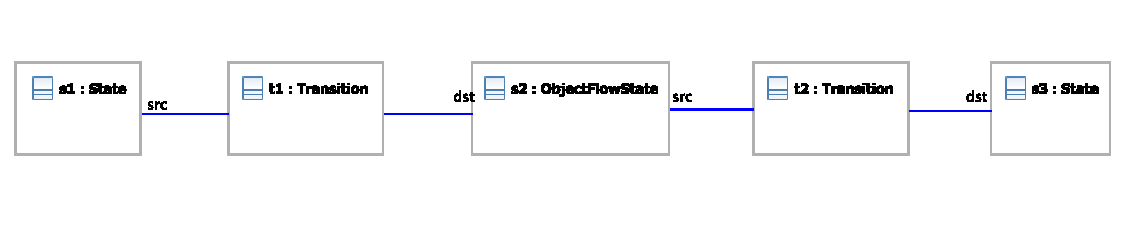
\includegraphics[height=2.5cm]{6.Evaluation/images/ttc/core_before.pdf}
	}
	\subfigure[Equivalent ObjectFlow structure in UML 2.2]
	{
	    \label{fig:ofs_to_flow_after}
	    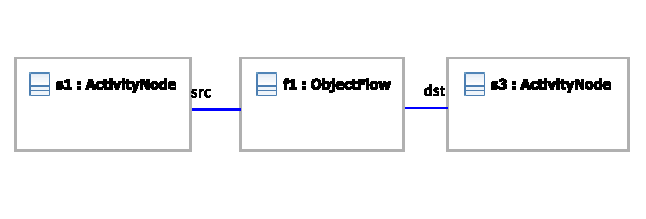
\includegraphics[height=2.5cm]{6.Evaluation/images/ttc/ext_after.pdf}
	}
	\caption{Migrating Actions for Extension 1}
\label{fig:ofs_to_flow}
\end{figure}

\subsubsection{Extension 2: Concrete Syntax}
\label{sub:concrete_syntax}
The second extension relates to the appearance of activity diagrams. The UML specifications provide no formally defined metamodel for the concrete syntax of UML diagrams. However, some UML tools store diagrammatic information in a structured manner using XML or a modelling tool. For example, the Eclipse UML 2 tools\footnote{\url{http://www.eclipse.org/modeling/mdt/?project=uml2tools}} store diagrams as GMF \cite{gronback09emp} diagram models.

Submissions were invited to explore the feasibility of migrating the concrete syntax of the activity diagram shown in Figure~\ref{fig:activity} to the concrete syntax in their chosen UML 2 tool. To facilitate this, the case resources included an ArgoUML project\footnote{\url{http://argouml.tigris.org/}} containing the activity diagram shown in Figure~\ref{fig:activity}.

\subsubsection{Extension 3: XMI}
\label{sub:xmi}
The UML specifications \cite{uml14,uml22} indicate that UML models should be stored using XMI. However, because XMI has evolved at the same time as UML, UML 1.4 tools most likely produce XMI of a different version to UML 2.2 tools. For instance, ArgoUML produces XMI 1.2 for UML 1.4 models, while the Eclipse UML2 tools produce XMI 2.1 for UML 2.2.

As an extension to the core task, submissions were invited to consider how to migrate a UML 1.4 model represented in XMI 1.x to a UML 2.1 model represented in XMI 2.x. To facilitate this, the UML 1.4 model shown in Figure~\ref{fig:activity} was made available in XMI 1.2 as part of the case resources.

Following the submission of the case, Tom Morris, the project leader for ArgoEclipse and a committer on ArgoUML, encouraged solutions to consider the extension described above. ArgoUML cannot, at present, migrate models from UML 1 to UML 2.  On the TTC forums, Morris stated that ``We have nothing available to fill this hole currently, so any contributions would be hugely valuable.  Not only would achieve academic fame and glory from the contest, but you'd get to see your code benefit users of one of the oldest (10+ yrs) open source UML modeling tools.'' \footnote{\url{http://www.planet-research20.org/ttc2010/index.php?option=com_community&view=groups&task=viewdiscussion&groupid=4&topicid=20&Itemid=150} (registration required)}

\subsection{Model Migration Solution in Epsilon Flock}
\label{subsec:ttc_solution}
This section describes a Flock solution for migrating UML activity diagrams in response to the evolution described above. The solution was developed by the author, and, at the workshop, compared with migration strategies written in other languages. The workshop participants and organisers rated each tool.

The Flock migration strategy was developed in an iterative and incremental manner, using the following process, starting with an empty migration strategy:

\begin{enumerate}
	\item Execute Flock on the original model, producing a migrated model.
	\item Compare the migrated model with the reference model provided in the case resources.
	\item Change the Flock migration strategy.
	\item Repeat until the migrated and reference models were the same.
\end{enumerate}

The remainder of this section presents the Flock solution in an incremental manner. The code listings in this section show only those rules relevant to the iteration being discussed.

\subsubsection{Actions, Transitions and Final States}
Development of the migration strategy began by executing an empty Flock migration strategy on the original model. Because Flock automatically copies model elements that have not been affected by evolution, the resulting model contained \texttt{Ps\-eu\-do\-st\-at\-e}s and \texttt{Tr\-an\-si\-ti\-on}s, but none of the \texttt{Ac\-ti\-onSt\-a\-te}s from the original model. In UML 2.2 activities, \texttt{Op\-aq\-ueAc\-ti\-on}s replace \texttt{Ac\-ti\-onSt\-a\-te}s. Listing~\ref{lst:actions} shows the Flock code for changing \texttt{Ac\-ti\-onSt\-a\-te}s to corresponding \texttt{Op\-aq\-ueAc\-ti\-on}s.

\begin{lstlisting}[caption=Migrating Actions, label=lst:actions, language=Flock]
migrate ActionState to OpaqueAction
\end{lstlisting}

Next, similar rules were added to migrate instances of \texttt{FinalState} to instances of \texttt{ActivityFinalNode} and to migrate instances of \texttt{Transition} to \texttt{ControlFlow}, as shown in Listing~\ref{lst:final_states}.

\begin{lstlisting}[caption=Migrating FinalStates and Transitions, label=lst:final_states, language=Flock]
migrate FinalState to ActivityFinalNode
migrate Transition to ControlFlow
\end{lstlisting}

\subsubsection{Pseudostates}
Development continued by selected further types of state that were not present in the migrated model, such as \texttt{Ps\-eu\-do\-st\-at\-es}s, which are not used in UML 2.2 activities. Instead, UML 2.2 activities use specialised \texttt{No\-de}s, such as \texttt{In\-it\-ialNo\-de}. Listing~\ref{lst:pseudostates} shows the Flock code used to change \texttt{Ps\-eu\-do\-st\-a\-te}s to corresponding \texttt{No\-de}s.

\begin{lstlisting}[caption=Migrating Pseudostates, label=lst:pseudostates, language=Flock]
migrate Pseudostate to InitialNode  when: original.kind = Original!PseudostateKind#initial
migrate Pseudostate to DecisionNode when: original.kind = Original!PseudostateKind#junction
migrate Pseudostate to ForkNode     when: original.kind = Original!PseudostateKind#fork
migrate Pseudostate to JoinNode     when: original.kind = Original!PseudostateKind#join
\end{lstlisting}

\subsubsection{Activities}
In UML 2.2, \texttt{Ac\-ti\-vi\-ty}s no longer inherit from state machines. As such, some of the features defined by \texttt{Ac\-ti\-vi\-ty} have been renamed. Specifically, \texttt{tr\-an\-si\-ti\-o\-ns} has become \texttt{ed\-g\-es} and \texttt{par\-ti\-ti\-o\-ns} has become \texttt{gr\-o\-sup}. Furthermore, the states (or nodes in UML 2.2 parlance) of an \texttt{Ac\-ti\-vi\-ty} are now contained in a feature called \texttt{nodes}, rather than in the \texttt{su\-bv\-er\-t\-ex} feature of a composite state accessed via the \texttt{top} feature of \texttt{Ac\-ti\-vi\-ty}. The Flock migration rule shown in Listing~\ref{lst:activities} captured these changes.

\begin{lstlisting}[caption=Migrating ActivityGraphs, label=lst:activities, language=Flock]
migrate ActivityGraph to Activity {
	migrated.edge  = original.transitions.equivalent();
	migrated.group = original.partition.equivalent();
	migrated.node  = original.top.subvertex.equivalent();
}
\end{lstlisting}

Note that the rule in Listing~\ref{lst:activities} used the built-in \texttt{eq\-ui\-va\-le\-nt} operation to find migrated model elements from original model elements. As discussed in Section~\ref{sec:flock}, the \texttt{equ\-iv\-al\-e\-nt} operation invokes other migration rules where necessary and caches results to improve performance.

Next, a similar rule for migrating \texttt{Gu\-ar\-d}s was added. In UML 1.4, the the \texttt{gu\-a\-rd} feature of \texttt{Tr\-an\-si\-ti\-on} references a \texttt{Gu\-a\-rd}, which in turn references an \texttt{Ex\-pr\-es\-si\-on} via its \texttt{ex\-pr\-es\-si\-on} feature. In UML 2.2, the \texttt{gu\-a\-rd} feature of \texttt{Tr\-an\-si\-ti\-on} references an \texttt{Op\-aq\-ueEx\-pr\-es\-si\-on} directly. Listing~\ref{lst:guards} captures this in Flock.

\begin{lstlisting}[caption=Migrating Guards, label=lst:guards, language=Flock]
migrate Guard to OpaqueExpression {
	migrated.body.add(original.expression.body);
}

\end{lstlisting}


\subsubsection{Partitions}
In UML 1.4 activity diagrams, \texttt{Pa\-rt\-it\-i\-on} specifies a single containment reference for its \texttt{co\-nt\-en\-ts}. In UML 2.2 activity diagrams, partitions have been renamed to \texttt{ActivityPartition}s and specify two containment features for their contents, \texttt{ed\-g\-es} and \texttt{no\-d\-es}. Listing~\ref{lst:partitions} shows the rule used to migrate \texttt{Pa\-rt\-it\-i\-on}s to \texttt{Ac\-ti\-vi\-tyPa\-rt\-it\-i\-on}s in Flock. The body of the rule shown in Listing~\ref{lst:partitions} uses the \emph{collect} operation to segregate the \texttt{co\-nt\-en\-ts} feature of the original model element into two parts.

\begin{lstlisting}[caption=Migrating Partitions, label=lst:partitions, language=Flock]
migrate Partition to ActivityPartition {
	migrated.edges = original.contents.collect(e:Transition | e.equivalent());
	migrated.nodes = original.contents.collect(n:StateVertex | n.equivalent());	
}
\end{lstlisting}


\subsubsection{ObjectFlows}
Finally, two rules were written for migrating model elements relating to object flows. In UML 1.4 activity diagrams, object flows are specified using \texttt{Ob\-je\-ctFl\-owSt\-a\-te}, a subtype of \texttt{St\-at\-eVe\-rt\-ex}. In UML 2.2 activity diagrams, object flows are modelled using a subtype of \texttt{ObjectNode}. In UML 2.2 flows that connect to and from \texttt{Ob\-je\-ctNo\-de}s must be represented with \texttt{Ob\-je\-ctFl\-ow}s rather than \texttt{Co\-nt\-rolFl\-ow}s.

Listing~\ref{lst:objectflows} shows the Flock rule used to migrate \texttt{Tr\-an\-si\-ti\-on}s to \texttt{Ob\-je\-ctFl\-ow}s. The rule applies for \texttt{Tr\-an\-si\-ti\-on}s whose source or target \texttt{St\-at\-eVe\-rt\-ex} is of type \texttt{Ob\-je\-ctFl\-owSt\-ate}.

\begin{lstlisting}[caption=Migrating ObjectFlows, label=lst:objectflows, language=Flock]
migrate ObjectFlowState to ActivityParameterNode

migrate Transition to ObjectFlow when: original.source.isTypeOf(ObjectFlowState) or original.target.isTypeOf(ObjectFlowState)
\end{lstlisting}

In addition to the core task, the Flock solution also approached two of the three extensions described in the case (Section~\ref{subsec:ttc_case}). The solutions to the extensions are now discussed.

\subsubsection{Alternative ObjectFlowState Migration Semantics}
The first extension required submissions to consider an alternative migration semantics for \texttt{Ob\-je\-ctFl\-owSt\-a\-te}, in which a single \texttt{Ob\-je\-ctFl\-ow} replaces each \texttt{Ob\-je\-ctFl\-owSt\-a\-te} and any connected \texttt{Tr\-an\-si\-ti\-on}s.

Listing~\ref{lst:objectflows2} shows the Flock source code used to migrate \texttt{Ob\-je\-ctFl\-owSt\-at\-es} (and connecting \texttt{Tr\-an\-si\-ti\-on}s) to a single \texttt{Ob\-je\-ctFl\-ow}. This rule was used instead of the two rules defined in Listing~\ref{lst:objectflows}. In the body of the rule shown in Listing~\ref{lst:objectflows2}, the \texttt{so\-ur\-ce} of the \texttt{Tr\-an\-si\-ti\-on} is copied directly to the \texttt{so\-u\-rce} of the \texttt{Ob\-je\-ctFl\-ow}. The \texttt{ta\-rg\-et} of the \texttt{Ob\-je\-ctFl\-ow} is set to the target of the first outgoing \texttt{Tr\-an\-si\-ti\-on} from the \texttt{Ob\-je\-ctFl\-owSt\-a\-te}. 

\begin{lstlisting}[caption=Migrating ObjectFlowStates to a single ObjectFlow, label=lst:objectflows2, language=Flock]
migrate Transition to ObjectFlow when: original.target.isTypeOf(ObjectFlowState) {
	migrated.source = original.source.equivalent();
	migrated.target = original.target.outgoing.first.target.equivalent();
}
\end{lstlisting}

Because, in this alternative semantics, \texttt{Ob\-je\-ctFl\-owSt\-a\-te}s are represented as edges rather than nodes, the partition migration rule was changed such that \texttt{Ob\-je\-ctFl\-owSt\-a\-te}s were not copied to the \texttt{no\-des} feature of \texttt{Pa\-rt\-it\-i\-on}s. To filter out the \texttt{Ob\-je\-ctFl\-owSt\-a\-te}s, line 3 of Listing~\ref{lst:partitions} was changed to include a reject statement, as shown on line 3 of Listing~\ref{lst:partitions2}.

\begin{lstlisting}[caption=Migrating Partitions without ObjectFlowStates, label=lst:partitions2, language=Flock]
migrate Partition to ActivityPartition {
	migrated.edges = original.contents.collect(e:Transition | e.equivalent());
	migrated.nodes = original.contents.reject(ofs:ObjectFlowState | true).collect(n:Original!StateVertex | n.equivalent());	
}
\end{lstlisting}

The complete source code listing for the Flock migration strategy is provided in Section~\ref{subsec:uml_activity_diagrams}.

\subsubsection{XMI}
\label{sec:xmi}
The second extension required submissions to migrate an activity graph conforming to UML 1.4 and encoded in XMI 1.2 to an equivalent activity graph conforming to UML 2.2 and encoded in XMI 2.1. The core task did not require submissions to consider changes to XMI (the model storage representation), but, in practice, this is a challenge to migration, as noted by Tom Morris on the TTC forums\footnote{\url{http://www.planet-research20.org/ttc2010/index.php?option=com_community&view=groups&task=viewdiscussion&groupid=4&topicid=20&Itemid=150} (registration required)}.

As discussed in Section~\ref{sec:flock}, Flock extends and reuses \changed{``is built atop'' changed to ``extends and reuses''} Epsilon, which includes a model connectivity layer (EMC). EMC provides a common interface for accessing and persisting models. Currently, EMC supports EMF (XMI 2.x), MDR (XMI 1.x), and plain XML models. To support migration between metamodels defined in heterogeneous modelling frameworks, EMC was extended during the development of Flock to provide a conformance checking service.

Consequently, the migration strategy developed for the core task works for all of the types of model supported by EMC. To migrate a model encoded in XMI 1.2 rather than in XMI 2.1, the user must select a different option when executing the Flock migration strategy. Otherwise, no other changes are required.

\subsection{Comparison with other solutions}
At the workshop, solutions to the migration case described in Section~\ref{subsec:ttc_case} were presented. Each solution was allocated two opponents who highlighted weaknesses of each approach. Following the solution presentations and opposition statements, each solution was scored using the criteria described above: correctness, clarity, conciseness, appropriateness, tool maturity, reproducibility and number of extensions solved. Flock scored the highest average marks for four of seven criteria, and was awarded overall first prize. The remainder of this section discusses the scores in more detail, and summarises the opposition statements for Flock.

\subsubsection{Opposition Statements}
The opposition statements highlighted two weaknesses of Flock. Firstly, there is some duplicated code in Listing~\ref{lst:pseudostates}: the \texttt{migrate Pseudostate to ...} statement appears several times. The duplication exists because Flock only allows one-to-one mappings between original and evolved metamodel types. The conservative copy algorithm would need to be extended to allow one-to-many mappings to remove this kind of duplication.

Secondly, the body of Flock rules are specified in an imperative manner. Consequently, reasoning about the correctness of a migration strategy is arguably more difficult than in languages that use a purely declarative syntax. This point is discussed further in Section~\ref{sec:limitations}, which considers the limitations of the thesis.

\subsubsection{Scoring}
Flock was awarded the overall first prize and scored the highest average marks for five of the seven criteria outlined above. The overall ranking process is first described, and the remainder of the section discusses the score awarded to Flock for each of the criteria.

During the workshop, each tool developer presented their solution. The workshop participants and organisers awarded each solution an individual score for each of the seven criteria outlined above, and a total score (by summing the seven criteria scores). The overall ranking for each solution was calculated by taking the mean of the total scores. For example, Flock was awarded the scores shown in Table~\ref{tab:flock_scores}. (Note that Participants \#2 and \#3 did not award scores to Flock due to a conflict of interest). Appendix~\ref{TTCScores} presents the complete set of results.

Although Flock was awarded the overall first prize, few conclusions can be drawn from the rankings. The scores for each criterion were awarded on different scales (e.g. -2 to 2 for conciseness, and 0 to 2 for extensions) and the workshop organisers applied a weight to each criterion before calculating the totals (5 for correctness; 4 for tool maturity; 3 for conciseness, clarity, extensions, and appropriateness; and 2 for reproducibility). Clearly, the relative importance of each criterion may vary between migration cases, and between organisations. Therefore, the remainder of the discussion focusses on the per-criteria scores awarded to Flock and the other tools.

\begin{table}[tbp]
	\centering
	\begin{tabular}{|r|c|c|c|c|c|c|c|c|c|c|c|}
		\hline
		\textbf{Response \#} & \textbf{1} & \textbf{4} & \textbf{5} & \textbf{6} & \textbf{7} & \textbf{8} & \textbf{9} & \textbf{10} & \textbf{11} & \textbf{12} & \textbf{Mean} \\
		\hline
		\hline
		Correctness          & 0          & 1          & 1          & 1          & 0          & 0          & 1          & 1     
		        & 1           & 1           & \\
		\hline                                                                                                     
		Conciseness          & 1          & 2          & 2          & 1          & 1          & 1          & 0          & 1
		        & 2           & 1           & \\
		\hline                                                                                                     
		Clarity              & 1          & 1          & 1          & 0          & 1          & 1          & 1          & 1
		        & 1           & 1           & \\
		\hline                                                                                                     
		Extensions           & 2          & 2          & 2          & 1          & 2          & 2          & 2          & 2
		        & 2           & 1           & \\
		\hline                                                                                                     
		Appropriateness      & 1         & 2          & 2          & 1          & 2          & 1           & 1          & 2 
		        & 2           & 2           & \\
		\hline                                                                                                     
		Tool Maturity        & 0         & 0          & 0          & 1          & 0          & 0           & 1          & 1
		        & 0           & 1           & \\
		\hline                                                                                                     
		Reproducibility      & 1         & 1          & 1          & 1          & 1          & 1          & 1          & 1 
		        & 1           & 1           & \\
		\hline                                                                                                     
		\hline                                                                                                     
		Total                & 6         & 9          & 9          & 6          & 7          & 6          & 7          & 9 
		        & 9           & 8           & 7.6 \\
		\hline
	\end{tabular}
	\caption{TTC scores for Epsilon Flock (unweighted).}
	\label{tab:flock_scores}
\end{table}

\paragraph{Correctness} Each tool developer demonstrated the extent to which their solution performed a correct migration of activity diagrams according to the migration semantics described in the case description (Section~\ref{subsec:ttc_case}). The following scores could be awarded: -1 (probably doesn't work at all), 0 (cannot judge), 1 (works for one model), and 2 (works for more than one model). Flock received a mean score of 0.7, and was ranked seventh out of the nine solutions. Migration with Flock is specified with both imperative and declarative language constructs, while many of the other solutions use only declarative language constructs to specify the migration of UML activity diagrams and, hence, more could be said about the correctness of the solutions written in those languages.

\paragraph{Conciseness} Solutions were awarded one of the following scores for the conciseness of their migration strategies: -2 (very verbose), -1 (quite verbose), 0 (cannot judges), 1 (quite concise), and 2 (very concise). Flock received a mean score of 1.2, and was ranked first out of the nine solutions. Three of the solutions used general purpose languages (such as Java and Prolog), and these were ranked sixth, seventh and ninth. The other solutions used graph or model transformation languages, and, in general, scored more highly than those written in general-purpose languages.

\paragraph{Clarity} The extent to which the intention of the migration could be determined from the migration strategy was scored on the following scale: -1 (no idea how it works), 0 (some idea how it works), 1 (fully understand how it works). Flock received a mean score of 0.9, was ranked first out of the nine solutions, and there was little variation in the scores awarded to Flock (a score of 1 from eleven of the twelve responses, and a score of 0 from the remaining respondent). Tools tailored to model migration, such as Flock and COPE \cite{herrmannsdoerfer09cope}, and graph transformation languages, such as GrGen \cite{grgen} and MOLA \cite{mola}, were ranked the highest in this category.

\paragraph{Appropriateness} The suitability of the tool for migrating activity diagrams was assessed on the following scale: -2 (totally inappropriate), -1 (inappropriate), 0 (neutral), 1 (somewhat appropriate), 2 (perfect fit). Flock received a mean score of 1.6, and was ranked first out of the nine solutions. Again, tools tailored to model migration, such as Flock and COPE \cite{herrmannsdoerfer09cope}, and graph transformation languages, such as GrGen \cite{grgen} and MOLA \cite{mola}, were ranked the highest in this category.

\paragraph{Tool maturity} The maturity of each tool was discussed during the solution presentations, and the workshop participants were able to use eight of the nine solutions via a virtual machine. Scores were awarded on the following scale: -1 (prototype), 0 (average), 1 (good). Flock received a mean score of 0.4, and was ranked third out of the nine solutions. Fujaba \cite{fujaba} and GrGen \cite{grgen} were ranked first and second in this category, and are established transformation tools that were first reported in the literature in 2000 and 2007 respectively.

\paragraph{Reproducibility} Each developer was invited to configure a virtual machine with their tool and solution, and the workshop participants were invited to use each of the tools. A score of 1 was awarded if a working virtual machine image was provided by the tool developer, and 0 otherwise. Flock had a mean score of 1, and ranked joint first along with seven of the other tools. The virtual machine image for one of the tools did not work, and it was awarded a mean score of 0.

\paragraph{Extensions} Three extensions to the core task were described in Section~\ref{subsec:ttc_case}, and a point was awarded for approaching each additional task. Flock was awarded a mean score of 5.4, and ranked first of the nine solutions. Determining the extensions approached by a solution seems to be an objective task, but some tools were awarded different scores for the extensions criterion which is difficult to explain. For instance, the Flock solution (Section~\ref{subsec:ttc_solution}) approached two of the three extensions, but some of the participants awarded Flock only 1 point. Rather than analysing the scores, it is perhaps more interesting to note that the Flock solution was the only solution to approach the XMI extension, and similarly for Fujaba \cite{fujaba} and the concrete syntax extension. This might indicate that contemporary migration tools can be used to manage realistic metamodel changes, but lack some features that would be desirable in an industrial setting (namely, interoperability with several modelling technologies and co-migration of abstract and concrete syntax).

\subsection{Summary}
This section has discussed the way in which Flock was evaluated by participating in the 2010 edition of the Transformation Tools Contest (TTC). Flock was assessed by application to an example of migration from the UML and comparison with eight other model and graph transformation tools. Flock was awarded the overall first prize and ranked first in five of seven categories by the workshop participants and organisers. 

In addition to evaluating Flock, the work described in this section provides three further contributions. Firstly, the migration case submitted to TTC 2010, described in Section~\ref{subsec:ttc_case} provides a real-world example of co-evolution for use in future comparisons of model migration tools. The case is based on the evolution of UML, between versions 1.4 and 2.2. The migration strategy was devised by analysis of the UML specification, and by discussion between workshop participants.


Secondly, the Flock solution to the migration case (Section~\ref{subsec:ttc_solution}) demonstrates the way in which a migration strategy can be constructed using Flock. In particular, Section~\ref{subsec:ttc_solution} describes an iterative and incremental development process and indicates that an empty Flock migration strategy can provide a useful starting point for development.

Finally, Section~\ref{sec:flock} claims that Flock supports several modelling technologies. The solution described in Section~\ref{subsec:ttc_solution} demonstrates the way in which Flock can be used to migrate models over two modelling technologies: MDR (XMI 1.x) and EMF (XMI 2.x), and hence supports the claim made in Section~\ref{sec:flock}.